\documentclass[]{scrartcl}

\usepackage{geometry}
\geometry{a4paper,left=25mm,right=25mm, top=1cm, bottom=2cm} 
\usepackage[latin1]{inputenc}
\usepackage{amsmath}
\usepackage{amsfonts}
\usepackage{amssymb}
\usepackage{graphicx}
%\usepackage{subfig}
\usepackage{epstopdf}
\usepackage{nicefrac}
\usepackage{color}
%\usepackage{subfig}
\usepackage{stackengine}
\usepackage{svg}

\usepackage{subcaption}

\title{Report of results}

\date{\today}
\begin{document}
\maketitle

\section{Continuous Version}
\label{sec:cv}

ToDo



\section{Lattice Version}
\label{sec:lv}

So far for the lattice version the influence of the length of the system, the detection radius and absorbing walls on the mean first passage time have been examined. For all simulations the target has been centered and periodic boundary conditions were used except in the case of absorbing walls. Averages are taken over one million simulations.


\subsection{System length L}
\label{ssec:sysL}

To examine the influence of the system length on the mean first passage time the system length has been varied between 10 and 1000 lattice sites.

\begin{figure}[!hbt]
 \centering
 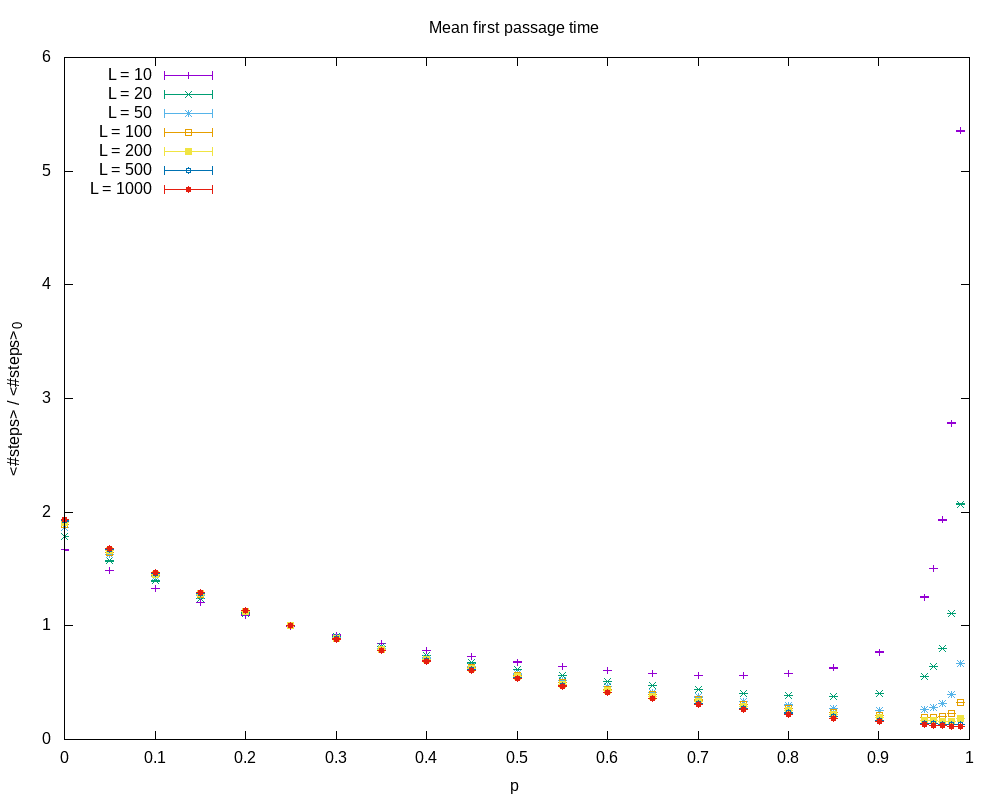
\includegraphics[width=0.8\textwidth]{./fig/sysL/fpt.png}
 \caption{Mean first passage time in dependency on the persistency for different system lengths. Mean first passage time has been rescaled by the mean first passage time for $p = 0.25$ which corresponds to diffusion.}\label{fig:sysL-fpt}
\end{figure}

As one can see in Figure \ref{fig:sysL-fpt} the minimum of the mean first passage time shifts to higher values of p (higher persistency) as the system length increases. Figure \ref{fig:sysL-p_opt} shows this more clearly and gives reason to assume that the optimal persistency approaches 1 in the limit of huge system sizes.

\begin{figure}[!hbt]
 \centering
 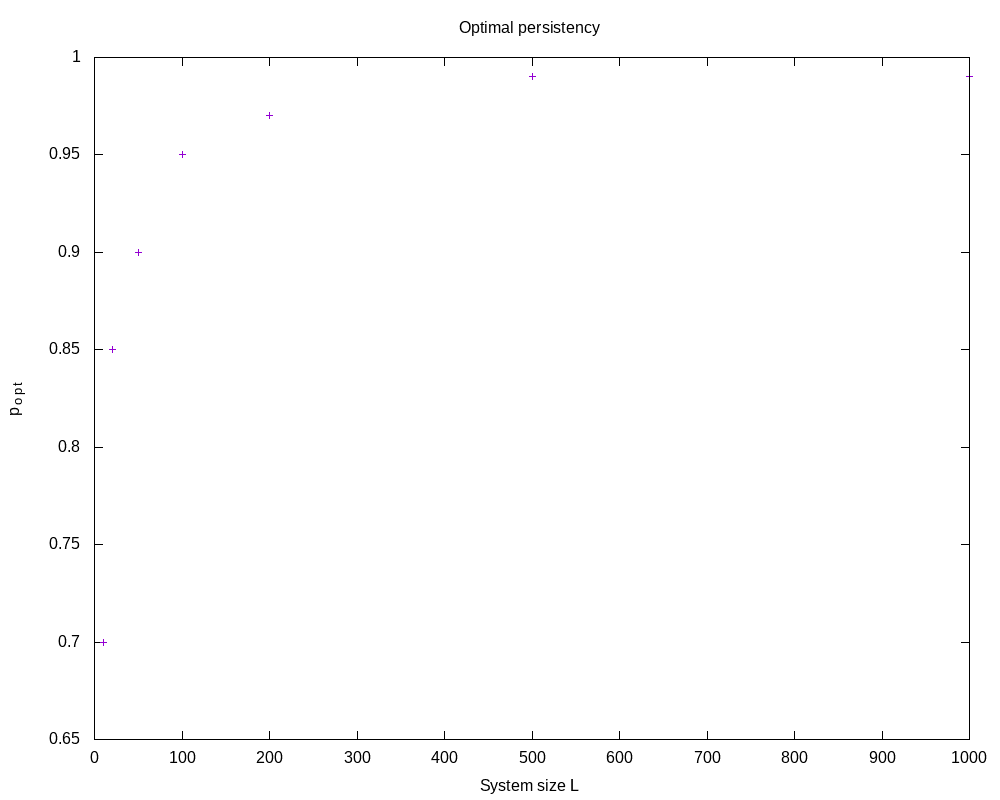
\includegraphics[width=0.8\textwidth]{./fig/sysL/p_opt.png}
 \caption{Optimal persistency in dependency on the system length.}
 \label{fig:sysL-p_opt}
\end{figure}

Furthermore, figure \ref{fig:sysL-p_opt-logscales} shows different logscales for the optimal persistency to prove that there is no easy mathematical law describing the dependency.
 
 \begin{figure}[!hbt]
\centering
% \captionsetup[subfigure]{justification=justified,singlelinecheck=false,labelformat=simple}
\begin{subfigure}{0.35\textwidth}
 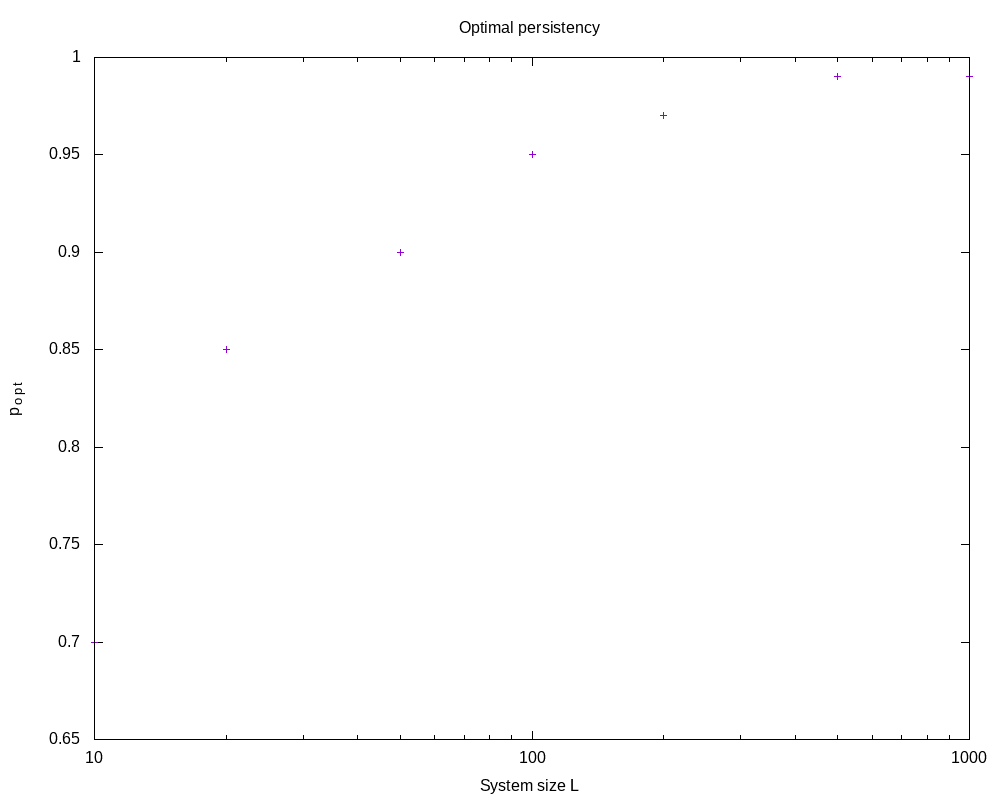
\includegraphics[width=\textwidth]{./fig/sysL/p_opt_logx.png}
  \subcaption{x logscale}
%  \label{}
\end{subfigure}
\begin{subfigure}{0.35\textwidth}
 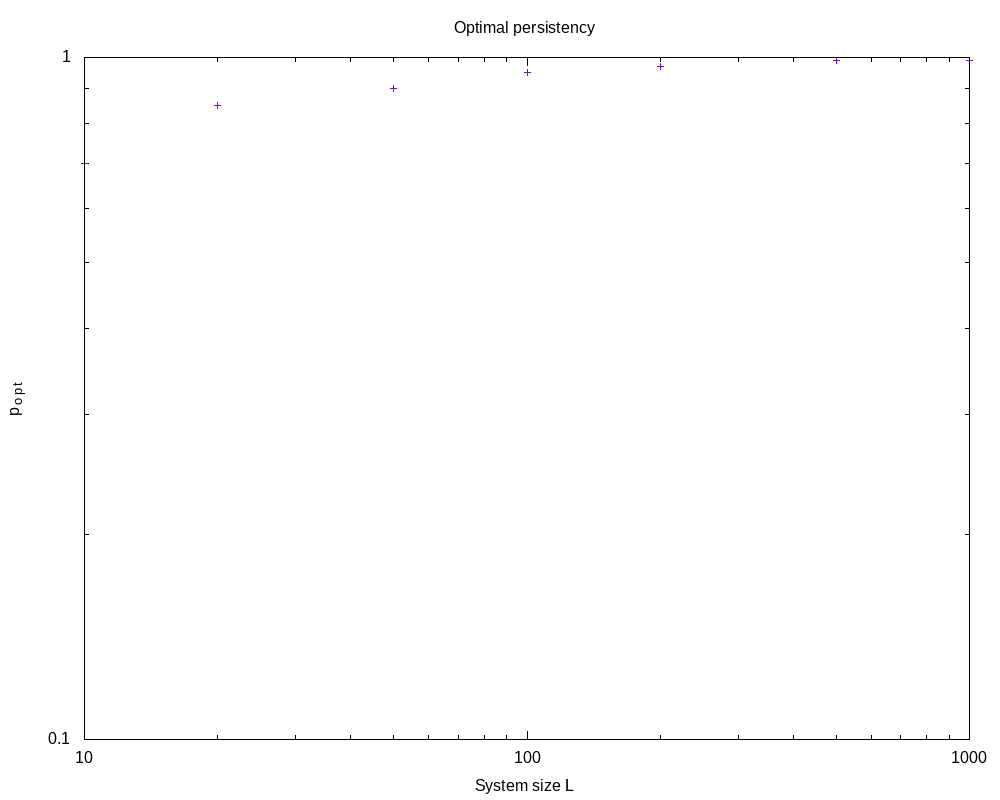
\includegraphics[width=\textwidth]{./fig/sysL/p_opt_logxy.png}
  \subcaption{xy logscale}
%  \label{}
\end{subfigure}
\begin{subfigure}{0.35\textwidth}
 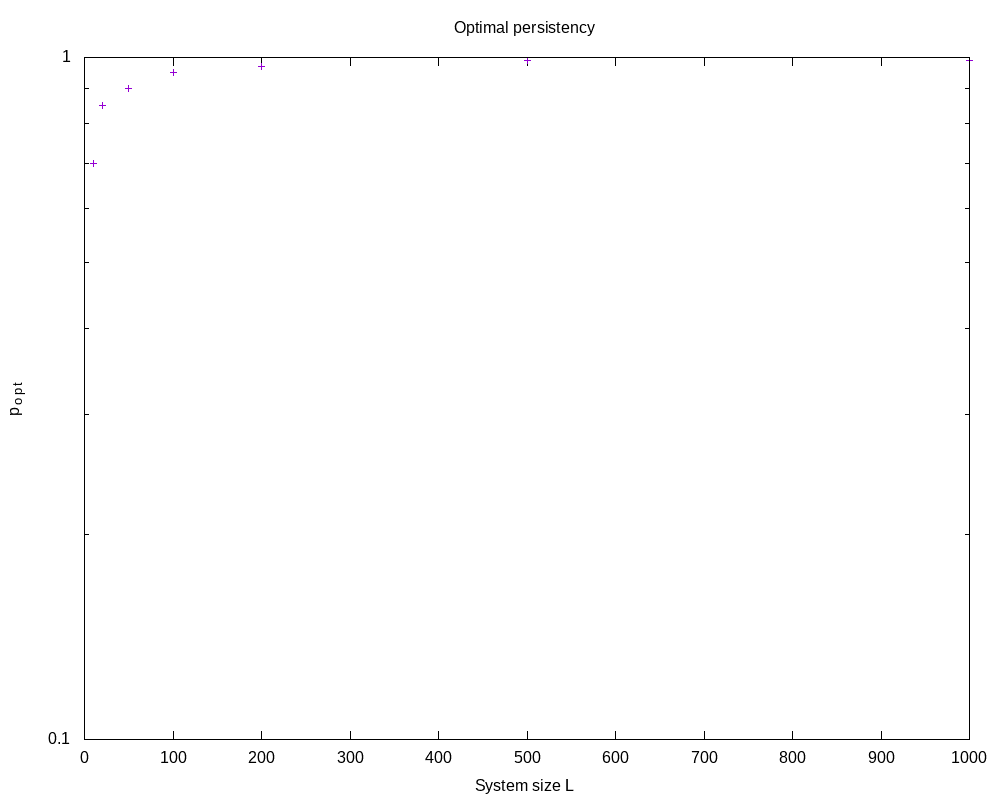
\includegraphics[width=\textwidth]{./fig/sysL/p_opt_logy.png}
  \subcaption{y logscale}
%  \label{}
\end{subfigure}
\caption{Different logscales for the optimal persistency in dependency on the system length.} 
\label{fig:sysL-p_opt-logscales}
\end{figure}


\subsection{Detection Radius D}
\label{ssec:detecR}

In order to check on the influence of the detection radius on the first passage time the system length has been chosen to be $L = 200$ and the detection radius has been varied between 1 and 20.

\begin{figure}[!hbt]
 \centering
 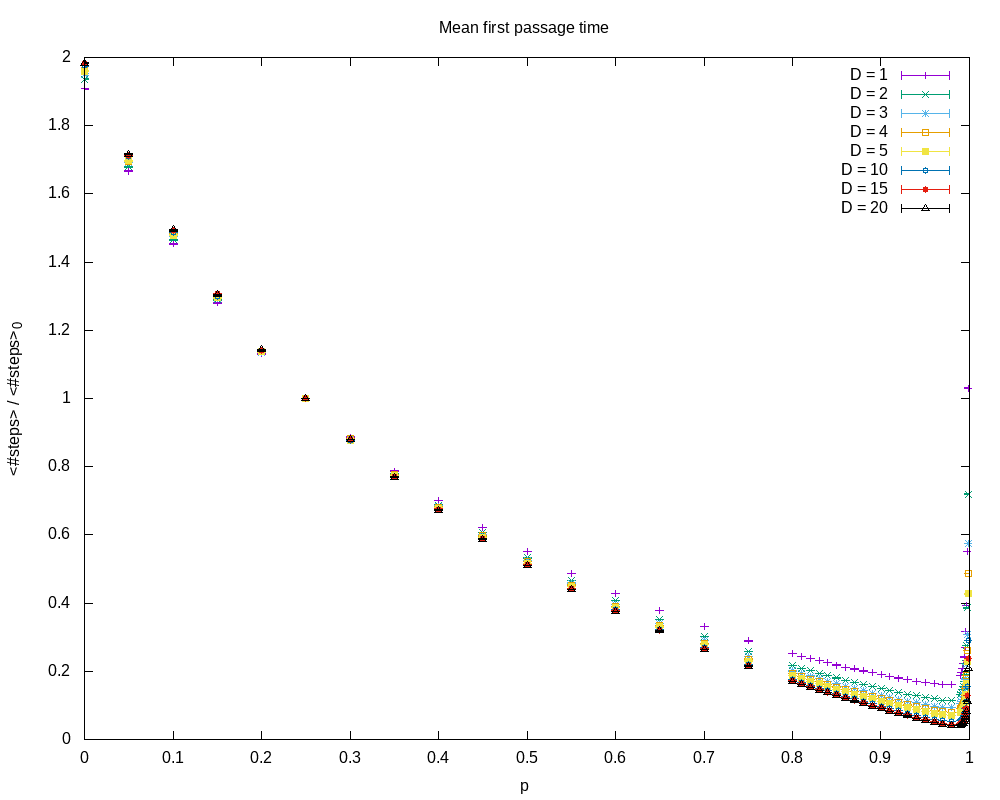
\includegraphics[width=0.8\textwidth]{./fig/detecR/fpt.png}
 \caption{Mean first passage time in dependency on the persistency for different detection radii. Mean first passage time has been rescaled by the mean first passage time for $p = 0.25$ which corresponds to diffusion.\label{fig:detecR-fpt}}
\end{figure}

The persistency value at the minimum of the mean first passage time seems to be unaffected by changes to the detection radius as can be seen in Figure \ref{fig:detecR-fpt} and Figure \ref{fig:detecR-opt_p}.

\begin{figure}[!hbt]
 \centering
 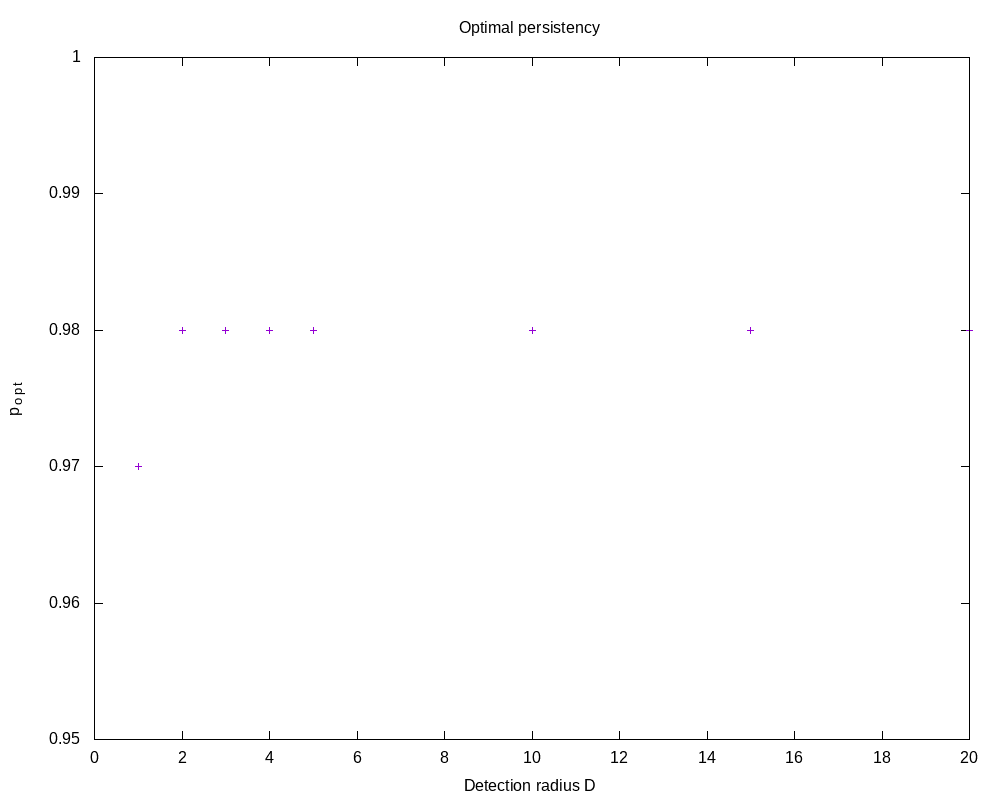
\includegraphics[width=0.8\textwidth]{./fig/detecR/p_opt.png}
 \caption{Optimal persistency in dependency on the detection radius.}
 \label{fig:detecR-opt_p}
\end{figure}


\subsection{Absorbing boundaries}
\label{ssec:alpha}

A third property to consider were the boundary conditions of the system. So far periodic boundaries have been examined. On the following pages the results of absorbing boundary conditions will be shown. Therefore, a new parameter $\alpha$ is introduced, which gives the probability of the searcher to be released from the absorbing wall in each timestep. Also the influence of the system length for absorbing boundaries will be shown. However, the detection radius is fixed to $D = 1$ in the following. The position of the target is also randomized for each single simulation.

 \begin{figure}[!hbt]
\centering
% \captionsetup[subfigure]{justification=justified,singlelinecheck=false,labelformat=simple}
\begin{subfigure}{0.45\textwidth}
 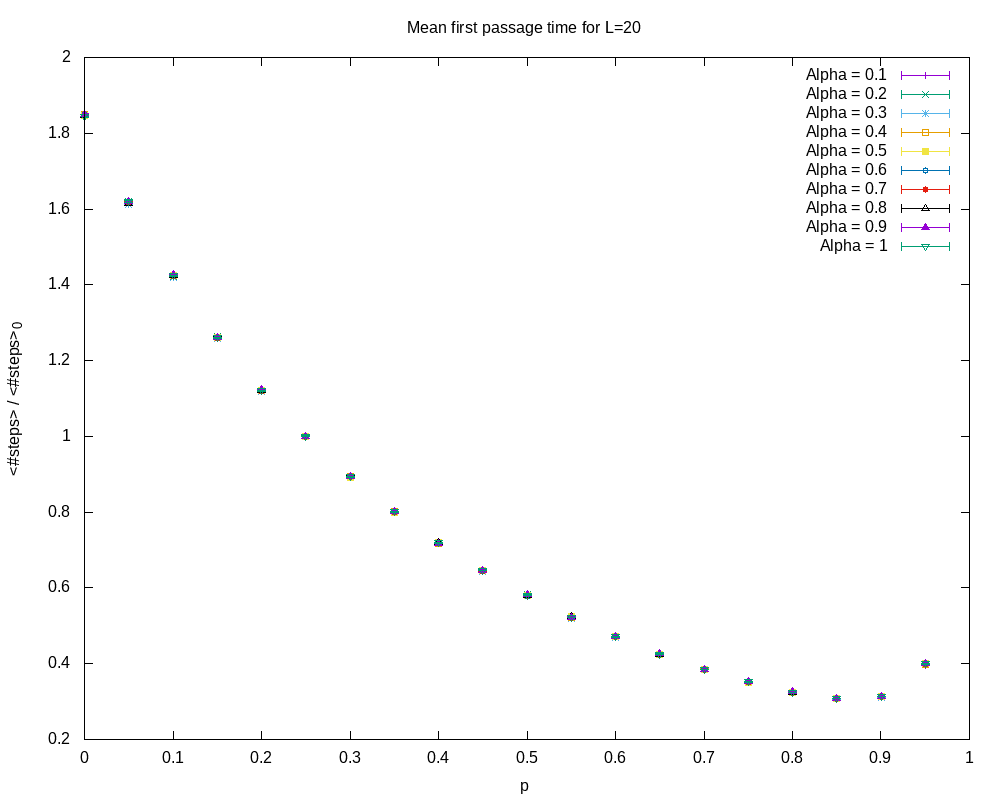
\includegraphics[width=\textwidth]{./fig/alpha/L=20/fpt.png}
  \subcaption{Rescaled MFPT}
%  \label{}
\end{subfigure}
\begin{subfigure}{0.45\textwidth}
 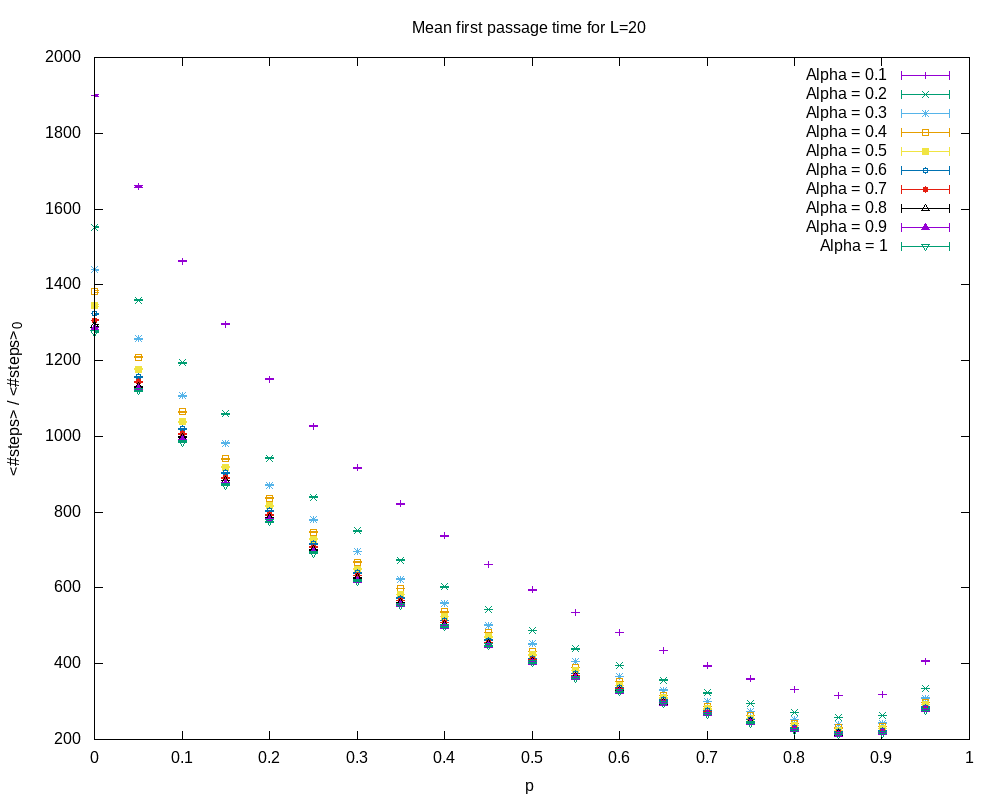
\includegraphics[width=\textwidth]{./fig/alpha/L=20/fpt2.png}
  \subcaption{MFPT}
%  \label{}
\end{subfigure}
\caption{Mean first passage time for system length $L = 20$ and absorbing boundary conditions for different parameters $\alpha$. (a) Mean first passage time rescaled by mfpt for $p = 0.25$. (b) Unscaled mfpt.} 
\label{fig:alpha-fpts20}
\end{figure}

 \begin{figure}[!hbt]
\centering
% \captionsetup[subfigure]{justification=justified,singlelinecheck=false,labelformat=simple}
\begin{subfigure}{0.45\textwidth}
 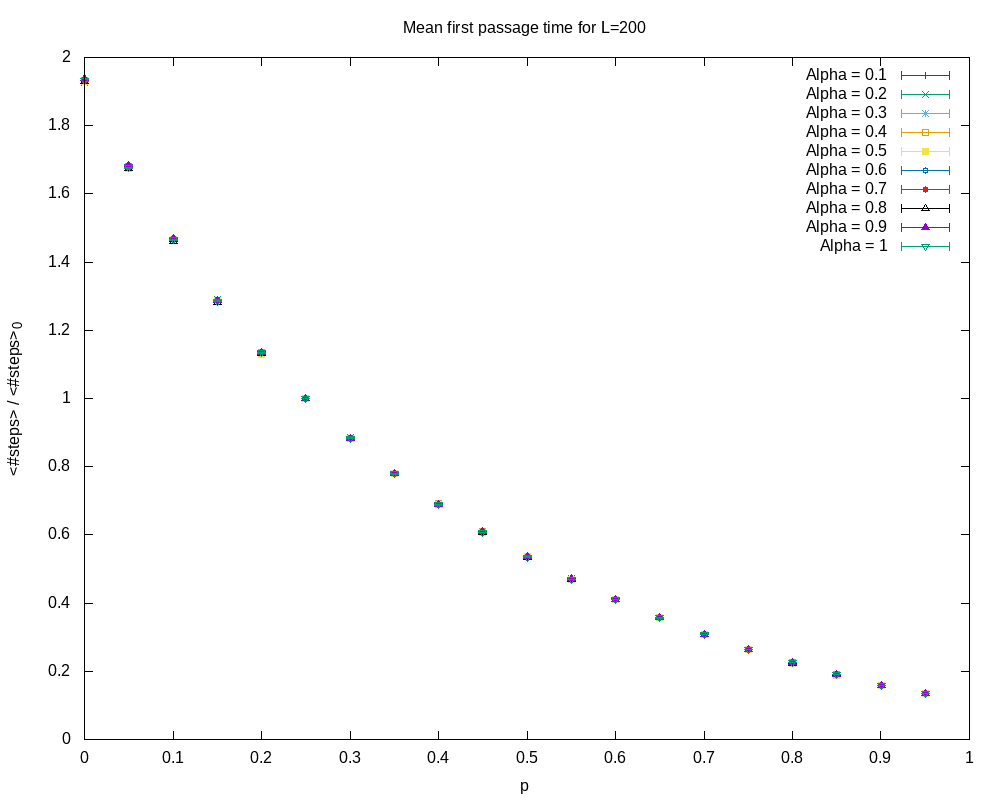
\includegraphics[width=\textwidth]{./fig/alpha/L=200/fpt.png}
  \subcaption{Rescaled MFPT}
%  \label{}
\end{subfigure}
\begin{subfigure}{0.45\textwidth}
 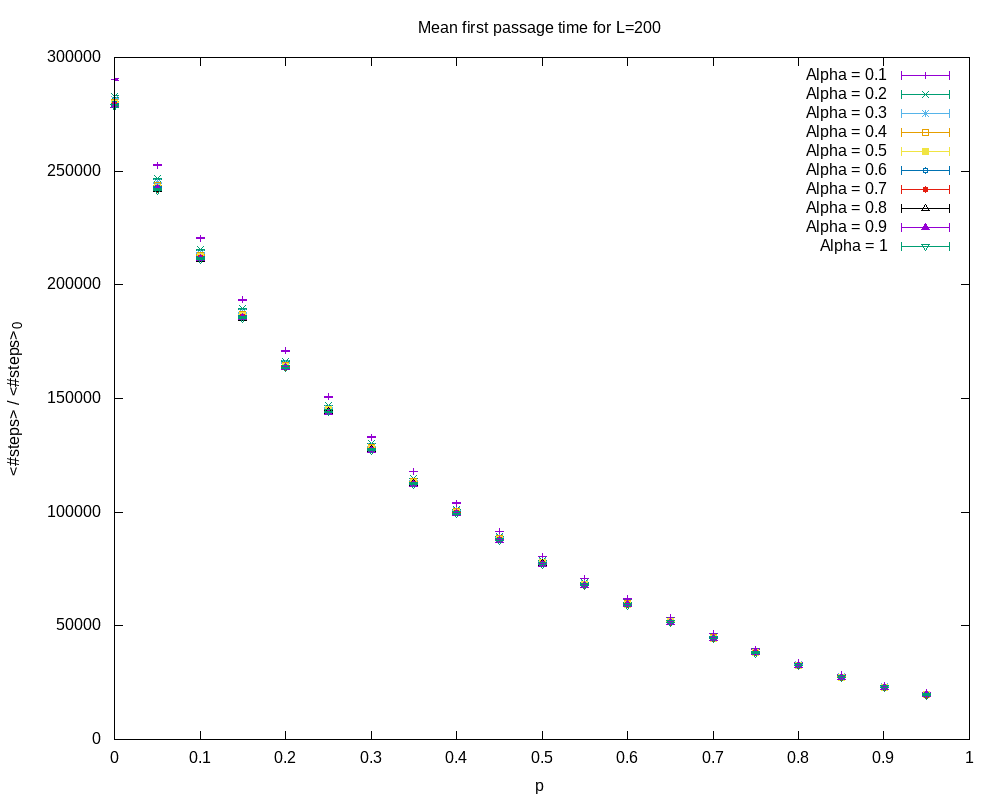
\includegraphics[width=\textwidth]{./fig/alpha/L=200/fpt2.png}
  \subcaption{MFPT}
%  \label{}
\end{subfigure}
\caption{Mean first passage time for system length $L = 200$ and absorbing boundary conditions for different parameters $\alpha$. (a) Mean first passage time rescaled by mfpt for $p = 0.25$. (b) Unscaled mfpt.} 
\label{fig:alpha-fpts200}
\end{figure}

As shown in Figure \ref{fig:alpha-fpts20} and Figure \ref{fig:alpha-fpts200} the influence of different system lengths is not altered in comparison to periodic boundary conditions (compare Figure \ref{fig:sysL-fpt}). Additionally, the variation of the parameter $\alpha$ does not influence the position of the optimal persistency at all. At first this is unexpected as one could assume that low $\alpha$ corresponds to long waiting times on the walls and therefore avoiding the walls would be beneficial. To gain further insight into this property, Figure \ref{fig:alpha-wallFreq} shows the average frequency of wall hits per step in a system of length $L = 200$ taken over one billion steps for three different values $\alpha$.

 \begin{figure}[!hbt]
\centering
% \captionsetup[subfigure]{justification=justified,singlelinecheck=false,labelformat=simple}
\begin{subfigure}{0.45\textwidth}
 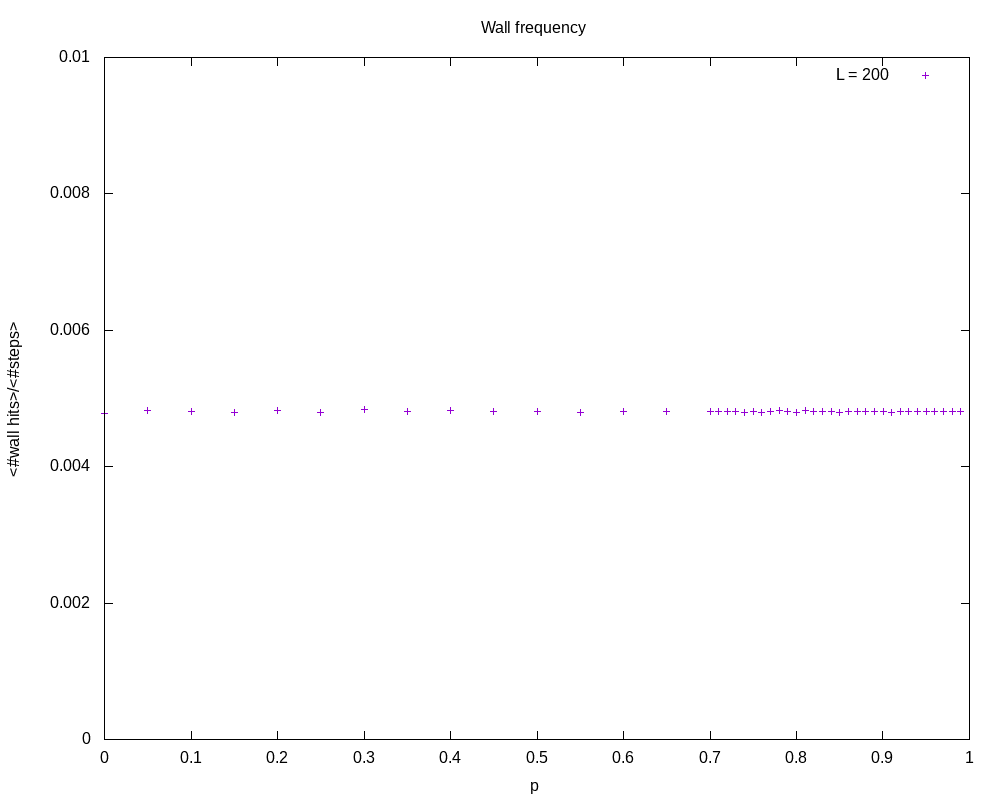
\includegraphics[width=\textwidth]{./fig/alpha/wallFreq/WF-alpha=01-rel.png}
  \subcaption{$\alpha = 0.1$}
%  \label{}
\end{subfigure}
\begin{subfigure}{0.45\textwidth}
 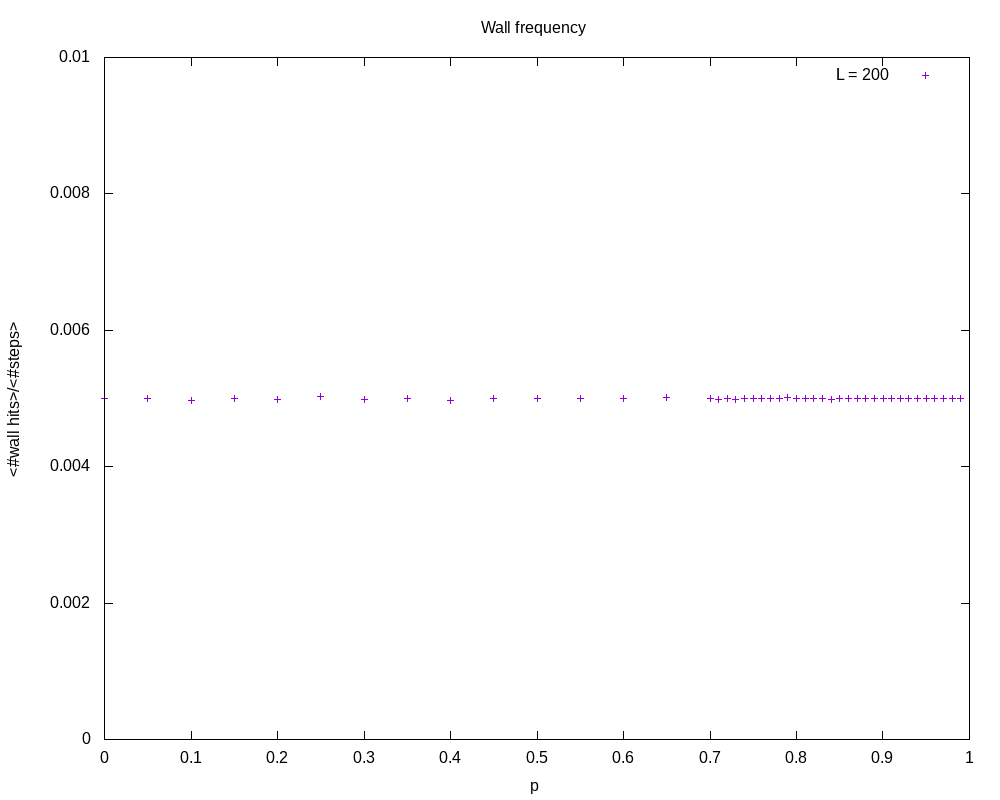
\includegraphics[width=\textwidth]{./fig/alpha/wallFreq/WF-alpha=05-rel.png}
  \subcaption{$\alpha = 0.5$}
%  \label{}
\end{subfigure}
\begin{subfigure}{0.45\textwidth}
 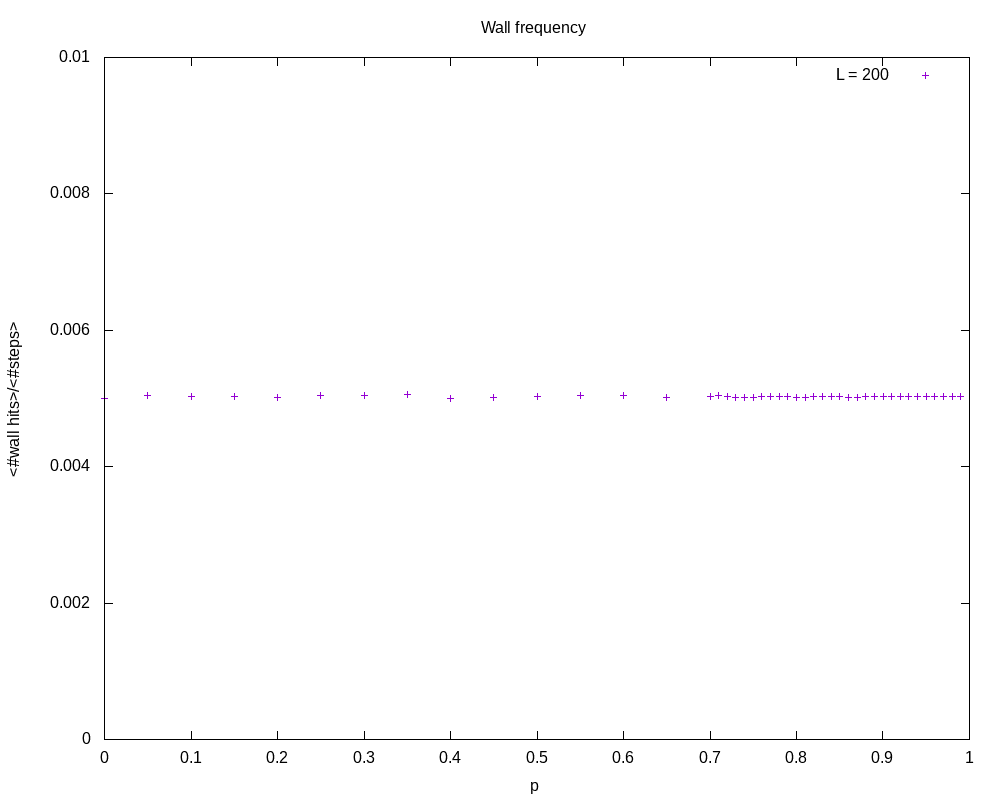
\includegraphics[width=\textwidth]{./fig/alpha/wallFreq/WF-alpha=1-rel.png}
  \subcaption{$\alpha = 1$}
%  \label{}
\end{subfigure}
\caption{Wall hit frequency per step for different values of $\alpha$ in a system of length $L = 200$.} 
\label{fig:alpha-wallFreq}
\end{figure}

With Figure \ref{fig:alpha-wallFreq} the results of Figure \ref{fig:alpha-fpts20} and Figure \ref{fig:alpha-fpts200} can be understood. As the amount of timesteps spent on the walls does not depend on the persistency but only on the total amount of time spent in the system, it is clear that the optimal persistency will remain the same when changing periodic boundaries to absorbing boundaries. The minimum will be even more clear in the case of absorbing boundaries since the smallest mfpt corresponds to lowest amount of timesteps spent on walls.

%  \begin{figure}[b]
%  \centering
%  \includegraphics[width=1.0\textwidth]{Figure1.eps}
%  \caption{aaa.}
%  \label{Fig1}
%  \end{figure} 
 

\end{document}
